\section{退出条件循环(\lstinline|do while|)}
\begin{frame}[fragile]\ft{\secname}
\begin{itemize}
\item
while循环和for循环都是入口条件循环,在每次执行循环之前先检查判断条件,这样循环中的语句可能一次也不执行。\\[0.1in]
\item 
\lstinline|do while|循环为退出条件循环,判断条件在执行循环之后进行检查,这可保证循环体中的语句至少被执行一次。
\end{itemize}
\end{frame}

\begin{frame}[fragile,allowframebreaks]\ft{\secname}
\lstinputlisting[language=c,numbers=left,frame=single]{ch06/code/do_while.c}

\end{frame}

\begin{frame}[fragile]\ft{\secname}
 \begin{lstlisting}[backgroundcolor=\color{red!10}]
To withdraw money from ATM.
Please enter the secret code number: 11
To withdraw money from ATM. 
Please enter the secret code number: 12
To withdraw money from ATM. 
Please enter the secret code number: 13
Congratulations! You are permitted!
\end{lstlisting}
\end{frame}

\begin{frame}[fragile,allowframebreaks]\ft{\secname}
若用while循环改写这段程序,代码会长一些。

\lstinputlisting[language=c,numbers=left,frame=single]{ch06/code/entry.c}

\end{frame}



\begin{frame}[fragile]\ft{\secname}
\begin{figure}
\centering
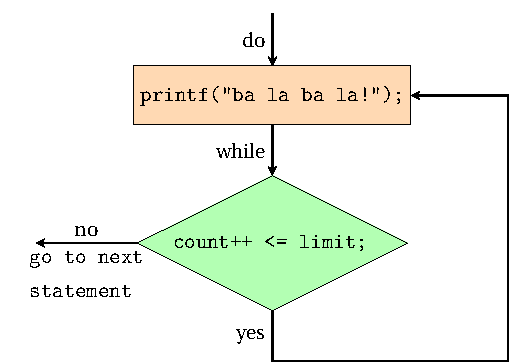
\includegraphics[width=4in]{ch06/images/do_while.pdf}
\end{figure}

\end{frame}

\begin{frame}[fragile]\ft{\secname}
\begin{lstlisting}[language=c,frame=single]
do {
        statements
} while (condition);

do 
        statement 
while (condition);
\end{lstlisting}

\end{frame}

\begin{frame}[fragile]\ft{\secname}

\begin{itemize}
\item
请注意\lstinline|do while|本身是一条语句,它需要一个结束的分号。\\[0.1in]
\item
应该把\lstinline|do while|\blue{仅用于}那些至少需要执行一次循环的情况。
\end{itemize}
\end{frame}



 
